\section{Эксперименты}

В этой части работы мы будем эксперименталено изучать статистическую неопределлённость различных сетевых структур. Перед нами стоят две задачи: понять, как отклонение от нормального распределения влияет на статистическую неопределённость и изучить статистическую неопределённость структур, построенных на основе новой меры близости - вероятности совпадения знаков.

Таким образом, экспериментальная часть будем состоять из двух частей. В первой части в качестве меры близости мы применяем выборочную корреляцию Пирсона, во второй - вероятность совпадения знаков. Каждая из частей эксперимента включает в себя оценку статистической неопределённости каждой из структур  при различных значениях коэффициента $r$ смешанного распределения. 
Список изучаемых структур придставлен ниже:
\begin{itemize}
	\item Максимального остовного дерева (maximum spanning tree)
	\item Рыночного графа (market graph)
	\item Максимальной клики на основе рыночного графа (maximum clique)
	\item Максимального независимого множества на основе рыночного графа (maximum independent set)
\end{itemize}


Как и в [ссылка на нашу статью] мы будем оценить статистическую неопределённость, основываясь на $\mathcal{E}(\mathcal{S},n)$-мере по следующему алгоритму: 
\begin{enumerate}
	\item Построить эталонную структуру на основе имеющихся данных
	\item Сгенерировать выборку доходностей акций $x_{1 1}, ..., x_{1 N}, ..., x_{n 1}, ..., x_{n N}$
	\item Рассчитать матрицу весов на основе меры близости и сгенерированных наблюдений
	\item Построить выборочную сеть
	\item В выборочной сети построить выборочную сетевую структуру
	\item Рассчитать долю ошибок I($\frac{X_1}{M_1}$) и II рода($\frac{X_2}{M_2}$) , а также общую долю ошибок $X$
	\item Повторить 500 раз шаги 2-5 и рассчитать среднее общей доли ошибок $X$. Полученное значение и будет являться оценкой меры $\mathcal{E}(\mathcal{S},n)$.
\end{enumerate}

Генерация выборки доходностей акций из смешанного распределения происходит следющим образом. В функцию генерации \verb|mixed_t_normal| кроме параметров, необходимых для генераторов из многомерного нормального распределения и многомерного распределения Стьюдента, описанных [ГДЕ-то Выше Наверно], передаётся число наблюдений $n$ и параметр $r \in [0,1]$, которые отвечает за то, какая часть из $n$ наблюдений будет сгенерирована из многомерного распределения Стьюдента. Оставшая часть будет сгенерирована из многомерного нормального распределения. Например, если при $n=100$ и $r=0.3$ 30 наблюдений будет сгенерировано из многомерного распределения Стьюдента, а 70 -из многомерного нормального распределения. При $r=0$ - все наблюдения будут сгенерированы из многомерного нормального распределения, а при  $r=1$ - все наблюдения будут сгенерированы из многомерного распределения Стьюдента. 

В качестве генератора многомерного нормального распределения  была использована функция \verb|random.multivariate_normal()| библиотеки Numpy. Генератор 
многомерного распределения Стьюдента реализует описанные в [Где-то сверху] выражения с помощью функций \verb|random.multivariate_normal()| и  \verb|random.chisquarel()| [ссылка на доку] библиотеки Numpy.

Рассмотрим более детально алгоритмы построения сетевых структур, а также специфику вычисления их статистической неопределённости.


Для построения максимального остовного дерева была использована  функция \verb|algorithms.tree.mst.maximum_spanning_tree()| библиотеки NetworkX[ссылка на доку]. Она реализует алгоритм Краскала[ссылка на алгоритм] построение минимального остовного дерева, который итеративно строит остовное дерево, на каждом шаге присоединяя ребро наименьшего веса, добавление которого не вызовет появления цикла. Алгоритм может быть использован и для поиска максимального остовного дерева,  выбирая на каждом шаге ребро наибольшего веса.

Остовное дерево, полученное как из эталонной, так и из выборочной сети, содержит $N$ вершин и $M_1 = M_2 = N-1$ рёбер. Так вершины соединяет только одно ребро, если существует ребёро $(i,j)$, которое ошибочно включено в выборочную структуру( $x^{i j}_1=1$), то существует и ребро  $(k,s)$, котороя ошибочно не включено в структуру ( $x^{k s}_2=1$) и наоборот. Таким образом, ошибки I и II рода эквиваленты, а общая доля ошибок может быть найдена как
\begin{equation}
X = \frac{1}{2}\left(\frac{X_1}{M_1} + \frac{X_2}{M_2}\right) = \frac{X_1 + X_2}{2(N-1)} = \frac{X_1}{N-1}
\end{equation}



Построение рыночного графа не потребовало использования никаких специальных алгоритмов. Рыночный граф легко получить, отфильтровав список рёбер по весу.
Для рыночного графа значения $M_1$ и $M_2$ по-прежнему константные, и равные $\binom{N}{2} - M$ и $M$ соответнственно, где $M$ - количество рёбер в эталонном рыночном графе с некоторым выбранным значением порога $\theta$, а $\binom{N}{2}$ - число всех возможных рёбер в графе с $N$ вершинами. Общая доля ошибок $X$ для рыночного графа равна:

\begin{equation}
X = \frac{1}{2}\left(\frac{X_1}{M_1} + \frac{X_2}{M_2}\right) = \frac{1}{2}\left(\frac{X_1}{\binom{N}{2} - M} + \frac{X_2}{M}\right)
\end{equation}


Максимальная клика и максимальное независимое множество строятся на основе полученного рыночного графа. Так как таких структур в графе может быть несколько, для оценки неопределённости, мы будем искать максимальную клику с максимальным весом (maximum clique with maximal weight) и максимальное независимое множество с минимальным весом (maximum independent set with minimal weight).  

Для поиска максимальной клики с максимальным весом в графе была использована функция \verb|algorithms.clique.find_cliques()| библиотеки NetworkX[ссылка на доку], которая возвращает список всех клик графа, каждая из которых является кортежем из вершин графа, входящих в клику. Реализация поиска основана на алгоритме Брона — Кербоша(ССЫЛКА) для поиска всех клик в неориентированном графе.Полученный список сортируется по размеру клик(числу элементов в кортеже), а потом из клик максимального размера выбирается клика с наибольшим весом. Вес клики определяется суммой весом рёбер рыночного графа, которые соединяют вершины, входящие в клику.


Так как максимальное независимое множество графа совпадает с максимальном кликой в обратном графе, поиск максимального независимого множество реализован через поиск максимальной клики в дополнении рыночного графа. Дополнением графа $G$ является граф, в котором две вершины являются смежными, если они не смежны в исходном графе. Множество вершин у исходного графа и его дополнения совпадают, а объединённые множества рёбер обоих графов составляет множество рёбер полного графа на этом множестве вершин. Дополнение графа также называют обратным графом (ССЫЛКА). Таким образом, чтобы найти максимальное независимое множество графа, можно применить описанный выше подход для поиска максимальной клики в дополнении рыночного графа, только вместо максимальной клики с наибольшим весом будем выбирать клику с наименьшим весом.

В отличие от максимального оставного дерева и рыночного графа значения $M_1$ уже не является константой, так как размер выборочной максимальной клики может изменяться. Теперь $M_1 = \binom{C_s}{2}$, а $M_2 = \binom{C_r}{2}$, где $C_s$ - число веришн в выборочной максимальной клике, а $C_r$ - число веришн в эталонной. Значение $C_r$ - константа.

\begin{equation}
X = \frac{1}{2}\left(\frac{X_1}{M_1} + \frac{X_2}{M_2}\right) = \frac{1}{2}\left(\frac{X_1}{\binom{C_s}{2}} + \frac{X_2}{\frac{X_2}{\binom{C_r}{2}}}\right)
\end{equation}


Алогоритм вычисления ошибок I и II рода ($X_1$ и $X_2$) одинаковый для каждой из структур. Он состоит в использовании функции  \verb|algorithms.operators.difference()| библиотеки NetworkX[ссылка на доку]. Эта функция принимает на вход два графа и возвращает граф с тем же множеством вершин  и множеством рёбер, которые содержатся в первом графе, но не содержатся во втором. У полученного графа мы считаем количество рёбер. Таким образом, передавая в функцию выборочную структуру первым аргументов, а эталонную вторым, мы получаем ошибку I рода. Передавая структуры в обратном порядке, получаем ошибку II рода


\subsection{Анализ эталонной сети}

Данными для эскперимента являются 470 наблюдений за $N=100$ акциями NASDAQ в период 2018-2019 годов. На основании этих данных, построим матрицу выборочной корреляции Пирсона $||\rho_{i j}||$ и матрицу вероятностей совпадения знаков, которые будут являться матрицами весов для эталонных сетей. К ним мы будем применять различные процедуры фильтрации и получать эталонные сетевые структуры, с помощью которых мы будем оценивать статистическую неопределённость.

Данные были загружены с помощью библиотеки Yahoo! Finance market data downloader [ссылка на доки]. Набор тикеров был получен путём веб-скрейпинга сайта http://eoddata.com.

Рассмотрим некоторые статистики эталонных сетевых структур с\textbf{ корреляцией Пирсона} в качестве меры близости. В таблице \ref{table:mg_size} отображена зависимость числа рёбер от выбранного порога $\theta$ в эталонном рыночном графе.

\begin{table}[h!]
\centering
\begin{tabular}{ |c|c|c|c|c|c|c|c|c|c| } 
 \hline
 $\theta$ & -1 & 0 & 0.1 & 0.2 & 0.3 & 0.4 & 0.5 & 0.6 & 0.7 \\ 
 \hline
 |E|	  & 4950 & 4584 & 3593 & 2282 & 1108 & 428 & 150 & 51 & 16\\ 
 \hline
\end{tabular}
\caption{Зависимость числа рёбер в рыночном графе от $\theta$}
\label{table:mg_size}
\end{table}


В таблице \ref{table:mis_clique_size} приведены размеры максимальной клики и максимального независимого множества в эталонном рыночном графе в зависимости от выбранного порога $\theta$.

\begin{table}[h!]
\centering
\begin{tabular}{ |c|c|c|c|c|c|c|c|c| } 
 \hline
 $\theta$ & 0 & 0.1 & 0.2 & 0.3 & 0.4 & 0.5 & 0.6 & 0.7 \\ 
 \hline
 N clique & 81 & 64 & 43 & 24 & 15 & 10 & 5 & 3\\ 
 \hline
 N mis    & 5  & 14 & 29 & 41 & 60 & 76 & 84 & 92\\ 
 \hline
\end{tabular}
\caption{Зависимость размеров структур от $\theta$}
\label{table:mis_clique_size}
\end{table}

На рисунке \ref{fig:ref_graph_p} изображён эталонный рыночный граф с порогом $\theta=0.5$, а также максимальная клики и максимальное независимое множество этого графа. Вершины, входящие в клику изображены синим цветом, входящие в независимое множество - красным.

\begin{figure}[H]
\centering
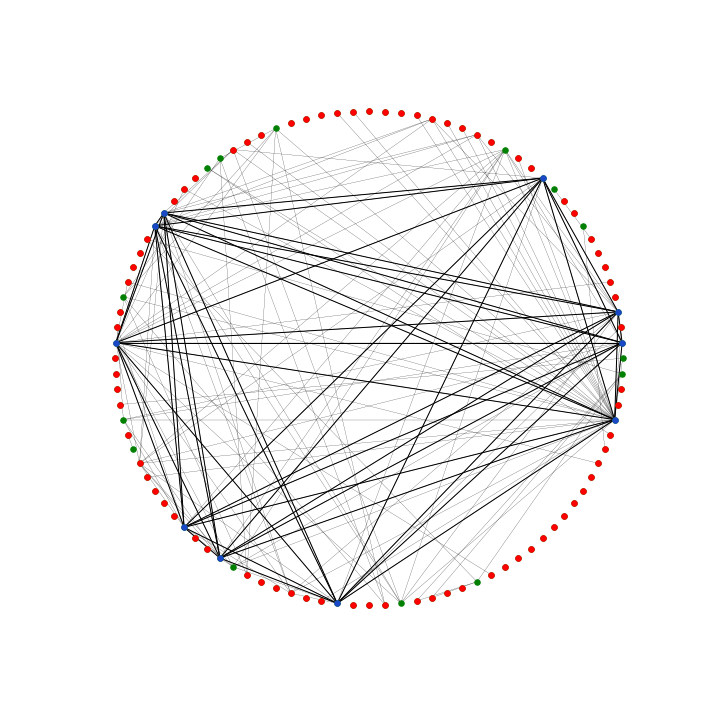
\includegraphics[scale=0.4]{ref_graph_p}
\caption{Эталонный рыночный граф с порогом $\theta=0.5$}
\label{fig:ref_graph_p}
\end{figure}



Теперь рассмотрим те же статистики эталонных сетевых структур, но с\textbf{ вероятностями совпадения знаков} в качестве меры близости. Порог $\theta$ преобразован в $\theta_\gamma$ согласно (\ref{eq:threshold}). 

В таблицах \ref{table:mg_size_sign} и \ref{table:mis_clique_size_sign} отображены зависимость числа рёбер от выбранного порога и  размеры максимальной клики и максимального независимого множества.

\begin{table}[h!]
\centering
\begin{tabular}{ |c|c|c|c|c|c|c|c|c|c|c|c| } 
 \hline
 $\theta$ & -1 & 0 & 0.1 & 0.2 & 0.3 & 0.4 & 0.5 & 0.6 & 0.7 & 0.8 & 0.9 \\ 
 \hline
  $\theta_\gamma$ & 0 & 0.5 & 0.53 & 0.56 & 0.6 & 0.63 & 0.67 & 0.7 & 0.75 & 0.8 & 0.86 \\ 
 \hline
 |E|	  & 4950 & 3906 & 3299 & 2341 & 1299 & 554 & 226 & 83 & 26 & 10 & 2 \\ 
 \hline
\end{tabular}
\caption{Зависимость числа рёбер в рыночном графе от $\theta$ и $\theta_\gamma$}
\label{table:mg_size_sign}
\end{table}


\begin{table}[h!]
\centering
\begin{tabular}{ |c|c|c|c|c|c|c|c|c|c|c| } 
 \hline
 $\theta$ & 0 & 0.1 & 0.2 & 0.3 & 0.4 & 0.5 & 0.6 & 0.7 & 0.8 & 0.9 \\ 
 \hline
  $\theta_\gamma$ & 0.5 & 0.53 & 0.56 & 0.6 & 0.63 & 0.67 & 0.7 & 0.75 & 0.8 & 0.86 \\ 
 \hline
 N clique & 73 & 55 & 37 & 25 & 16 & 10 & 5 & 4 & 3 & 2\\ 
 \hline
 N mis & 14  & 18 & 29 & 38 & 52 & 68 & 80 & 88 & 95 & 98\\ 
 \hline
\end{tabular}
\caption{Зависимость размеров структур от $\theta$ и $\theta_\gamma$}
\label{table:mis_clique_size_sign}
\end{table}



\subsection{Измерение неопределённости сетевых структур}

Для каждой из структур будем применять две меры неопределённости: корреляция Пирсона и вероятность совпадения знаков.

Для корреляции Пирсона основным экспериментом будет измерение доли общей ошибки в зависимости от числа наблюдений $n$ для различых параметром $r$. Таким образом, мы сможем изучить, как влияет на статистическую неопределённость отклонения от нормального распределения. 

Для вероятности совпадения знаков мы рассмотрим зависимость доли общей ошибки от параметра $r$ для различных значений параметра $r$ для различных значений числа наблюдений $n$. Так мы изучим влияние отклонения от нормального распределения на статистическую неопределённость структуры, построенной на вероятности совпадения знаков. Мы увидим, что подобного отклонения практически нет для любой из выбранных структур. Кроме того, мы сможем исследовать величину общей доли ошибки в зависимости от выбранной меры близости для выбранного значений $n$.

Для максимальной клики и максимального независимого множества помимо общей доли ошибки, будут также представлены доли ошибок I и II рода.

\subsubsection{Максимальное остовное дерево}

На рисунке \ref{exp:mst_10k_p} представлена


\subsubsection{Рыночный граф}
\subsubsection{Максимальная клика}
\subsubsection{Максимальное независимое множество}


